\subsection{Experimental Setup}

Evaluating a Doman DSE requires comparing over large set of applications, approaches and platforms. For the purpose of this paper, we use throughput improvement as a primary performance metric. It scales each application's throughput executing on the candidate platform over a pure SW implementation, quantifying speedup. We evaluate \newtext{DSS and} each version of \ga domain platforms, 
and compare against a full exhaustive search (where possible).

\newtext{The primary aim is to assess performance of all domain applications when executing on the candidate domain-specific platform} \figref{fig:DomainP}.
To understand the performance difference between domain-specific platform and application-specific platforms we build on the definitions in~\cite{zhang100ds}. Each application has an own OPTimal application-specific architecture (OPT) that maximizes the application throughput, see ~\figref{fig:OOP}. 
The OPT is obtained through (time consuming) exhaustive search. 
Executing each application in a domain on its own OPT yields the upper bound: \textbf{Own OPT Platform (OOP)} -- indicating the acceleration potential of a domain given a HW budget. In order to understand the penalty of application-specialization, we consider \textbf{Foreign OPT Platform (FOP)}, see \figref{fig:FOP}. Here, each application is evaluated multiple times, once on each platform in the pool of OPT (all but one being foreign to the application).



\begin{figure}[h]
	%\vspace{-5pt}
	\centering
		\subfloat[Domain Plat]{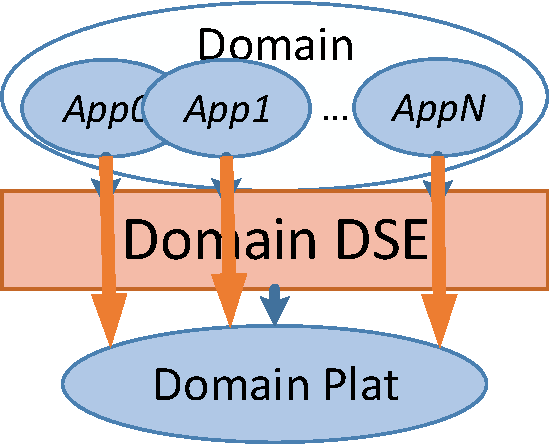
\includegraphics[width=.28\linewidth]{fig/pDomainP.pdf}\label{fig:DomainP}}
		\hfill
		\subfloat[OOP]{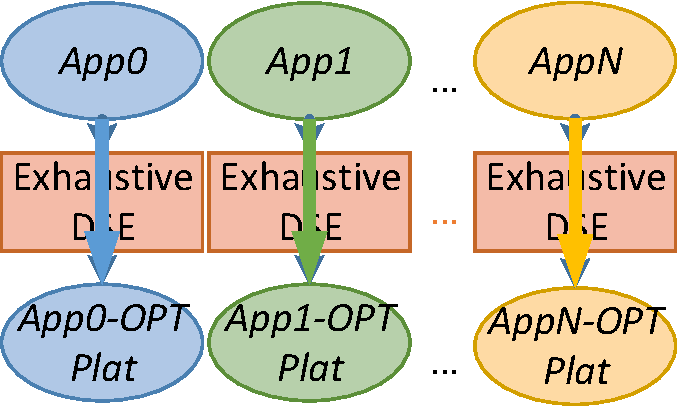
\includegraphics[width=.32\linewidth]{fig/pOOP.pdf}\label{fig:OOP}}
		\hfill
		\subfloat[FOP]{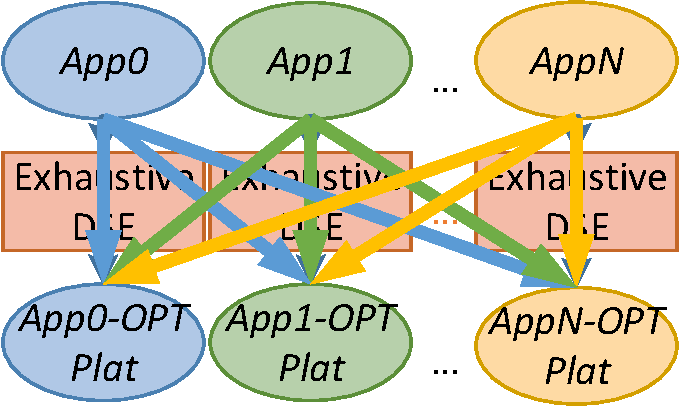
\includegraphics[width=.32\linewidth]{fig/pFOP.pdf}\label{fig:FOP}}
	%\vspace{-5pt}
	\caption{Experiments Settings}
	%\vspace{-4pt}
\end{figure}



We evaluate two domain types. The \textbf{OpenVX} domain (computer vision) has 35 function types and contains 40 applications from Intel \cite{Intel} and AMD \cite{AMD}, abstracted into data flow models. The \textbf{synthetic} domain is generated with 50 function types, containing 100 applications with a balance between processing and communication. 
%Performance is evaluated on automatically generated virtual platforms (SCE\cite{domer2008system}) capturing the abstract data flow model (SDF3\cite{stuijk2006sdf}) and architecture resources. 
The target platform contains a processor with N ACCs. Communication occurs on a 3R3W layer bus. The processing speedup on ACCs should be variable for different FTs, which could be implemented in different models, e.g. roofline model. For simplification, this paper just assumes ACC processing is 20x faster than SW. ACCs can communicate directly with each other~\cite{teimouri2016improving}.
